% !TeX root = ../tfg.tex
% !TeX encoding = utf8

\chapter{Homología persistente}

Este capítulo se dedica a la homología persistente, un concepto de gran relevancia en la topología computacional que proporciona herramientas poderosas para analizar y entender la estructura subyacente de los datos a través de múltiples escalas. Originada en los trabajos iniciales de matemáticos como Edelsbrunner, Letscher y Zomorodian \cite{edelsbrunner2002topological}, la homología persistente permite la identificación y el análisis de características topológicas que persisten a lo largo de variaciones en la escala en la que se observa.

Este capítulo se centrará en detallar los principios teóricos detrás de la homología persistente. En particular, estudiaremos en profundidad el Teorema de correspondencia, un resultado central en la teoría que muestra cómo transformar el nacimiento y muerte de las clases de homología en constructos algebraicos que se pueden analizar y manipular computacionalmente. Seguiremos como esquema principal los resultados de \cite{zomorodian2004computing} y \cite{dey2022computational}.

\section{Complejos de \u Cech y Vietoris-Rips}

La homología persistente es comúnmente empleada para analizar conjuntos de datos representados como nubes de puntos. Aunque la homología en sí de estos conjuntos puede no ser de gran interés debido a su simplicidad o falta de estructura topológica relevante, la homología persistente permite revelar información de interés mediante la construcción de estructuras topológicas construidas a partir de los datos.

En este contexto, los complejos de Čech y Vietoris-Rips se emplean frecuentemente para capturar la estructura topológica subyacente de las nubes de puntos. Estos complejos dotan de estructura de complejo simplicial a los datos, facilitando su representación, el estudio de su forma y sus características a múltiples escalas.
%
%\begin{definicion}
%	Sea \(X\) un espacio topológico y sea \(\mathcal{U} = \{U_v\}_{v \in V}\) un recubrimiento de \(X\). Llamaremos \textbf{nervio} de \(\mathcal{U}\) al complejo simplicial abstracto con conjunto de vértices \(V\) tal que la familia \(v_0, \dots, v_p\) genera un \(p\)-símplice si, y sólo si, \(U_{v_0} \cap \dots \cap U_{v_p} \neq \emptyset\). Lo notaremos por \(N(\mathcal{U})\).
%\end{definicion}
%
%\begin{teorema}[del Nervio]
%	Sea \(X\) un espacio topológico y sea \(\mathcal{U} = \{U_v\}_{v \in V}\) un recubrimiento por abiertos numerable de \(X\). Supongamos además que para todo subconjunto no vacío de vértices \(S \subseteq V\) tenemos que \(\bigcap_{s \in S} U_s\) es contráctil o vacío. Entonces \(N(\mathcal{U})\) es homotópicamente equivalente a \(X\).
%\end{teorema}
%\begin{proof}
%	Véase \cite{bjorner2003nerves}.
%\end{proof}

\begin{definicion}
	Sea \((X,d)\) un espacio métrico y sea \(V\) un subconjunto de puntos de \(X\). Definimos el \textbf{complejo de \u Cech} \(C(V, \varepsilon)\) como el nervio \(N(\mathcal{B}_\varepsilon)\), donde
	\[
		\mathcal{B}_\varepsilon = \{ B_{\varepsilon}(v) : v \in V \},
	\]
	siendo \(B_{\varepsilon}(v)\) la bola abierta de centro \(x\) y radio \(\varepsilon > 0\).
\end{definicion}

\begin{proposicion}
	El complejo de \u Cech \(C(V, \varepsilon)\) es un complejo simplicial abstracto.
\end{proposicion}
\begin{proof}
	Sea \( V = \{x_i\}_{i=1}^M \) un subconjunto de puntos en el espacio métrico \( X \). Definimos \( \mathcal{B}_\varepsilon = \{B_\varepsilon(x) : x \in V \} \) como un recubrimiento por abiertos de \( V \) para algún \(\varepsilon > 0\). Veamos que el nervio \( N(\mathcal{B}_\varepsilon) \) de \( \mathcal{B}_\varepsilon \) es el complejo abstracto cuyos vértices son los conjuntos \( B_\varepsilon(x) \) y los símplices se forman por colecciones de estos conjuntos que tienen intersecciones no vacías.
	
	Supongamos que tenemos un símplice \( \sigma = \{x_{i_1}, \ldots, x_{i_k}\} \) en \( N(\mathcal{B}_\varepsilon) \). Esto implica que
	\[
	\bigcap_{j=1}^k B_\varepsilon(x_{i_j}) \neq \emptyset.
	\]
	Consideremos ahora cualquier subconjunto de bolas de la forma  \(\{B_\varepsilon(x_{i_j})\}_{j \in J}\) donde \( J \subseteq \{1, \ldots, k\} \). Es claro que por ser $\sigma$ un símplice, 
	\[
	\bigcap_{j \in \{1, \ldots, k\} \setminus J} B_\varepsilon(x_{i_j}) \neq \emptyset,
	\]
	por lo que el conjunto de vértices restantes también forma un símplice en \( N(\mathcal{B}_\varepsilon) \). Por lo tanto, todas las caras de cualquier símplice \( \sigma \) son también símplices en \( N(\mathcal{B}_\varepsilon) \). Es decir, el nervio \( N(\mathcal{B}_\varepsilon) \) es cerrado bajo inclusiones.
	
	Dado que \( V \) es finito y cada símplice se define como un subconjunto de \( V \), entonces cada símplice sólo puede tener un número finito de subconjuntos. En consecuencia, el número de caras de cada símplice también es finito.
\end{proof}

Sin embargo, el complejo de \u Cech es costoso de obtener mediante métodos computaciones. En consecuencia, se propone el complejo de Vietoris-Rips:

\begin{definicion}
	Sea \((X,d)\) un espacio métrico y sea \(V\) un subconjunto de puntos de \(X\). Definimos el \textbf{complejo de Vietoris-Rips} \(VR(V,\varepsilon)\) como el complejo abstracto cuyo conjunto de vértices es \(V\), de forma que \(\{v_0, v_1, \dots v_p\} \subseteq V\) genera un \(p\)-símplice si, y sólo si, \(d(v_i,v_j) \leq \varepsilon\) para todo \(0 \leq i\), \(j \leq p\).
\end{definicion}

\begin{proposicion}
	El complejo de Vietoris-Rips \(VR(V,\varepsilon)\) es un complejo simplicial abstracto.
\end{proposicion}

\begin{proof}
	Primero veamos que el conjunto es cerrado bajo inclusiones. Supongamos que $\sigma = \{v_0, v_1, \dots, v_p\}$ es un $p$-símplice en $VR(V, \varepsilon)$. Por definición, esto significa que para todo $i, j$ tal que $0 \leq i, j \leq p$, se cumple que $d(v_i, v_j) \leq \varepsilon$. Consideremos ahora un subconjunto no vacío $\tau = \{v_{i_1}, v_{i_2}, \dots, v_{i_k}\} \subseteq \sigma$. Para cualquier par de índices $a, b$ con $1 \leq a, b \leq k$, los vértices $v_{i_a}$ y $v_{i_b}$ también cumplen que $d(v_{i_a}, v_{i_b}) \leq \varepsilon$, pues $\tau \subseteq \sigma$. Por lo tanto, $\tau$ es un $(k-1)$-símplice en $VR(V, \varepsilon)$.
	
	Por otro lado, cada $p$-símplice $\sigma$ en $VR(V, \varepsilon)$ es un subconjunto finito de $V$. El número de subconjuntos de cualquier conjunto finito es finito, y en particular, el número de subconjuntos de $\sigma$ es $2^{|\sigma|}$, donde $|\sigma|$ es el número de vértices en $\sigma$. En consecuencia, cada símplice en $VR(V, \varepsilon)$ tiene un número finito de caras.
\end{proof}

\begin{figure}
	\centering
	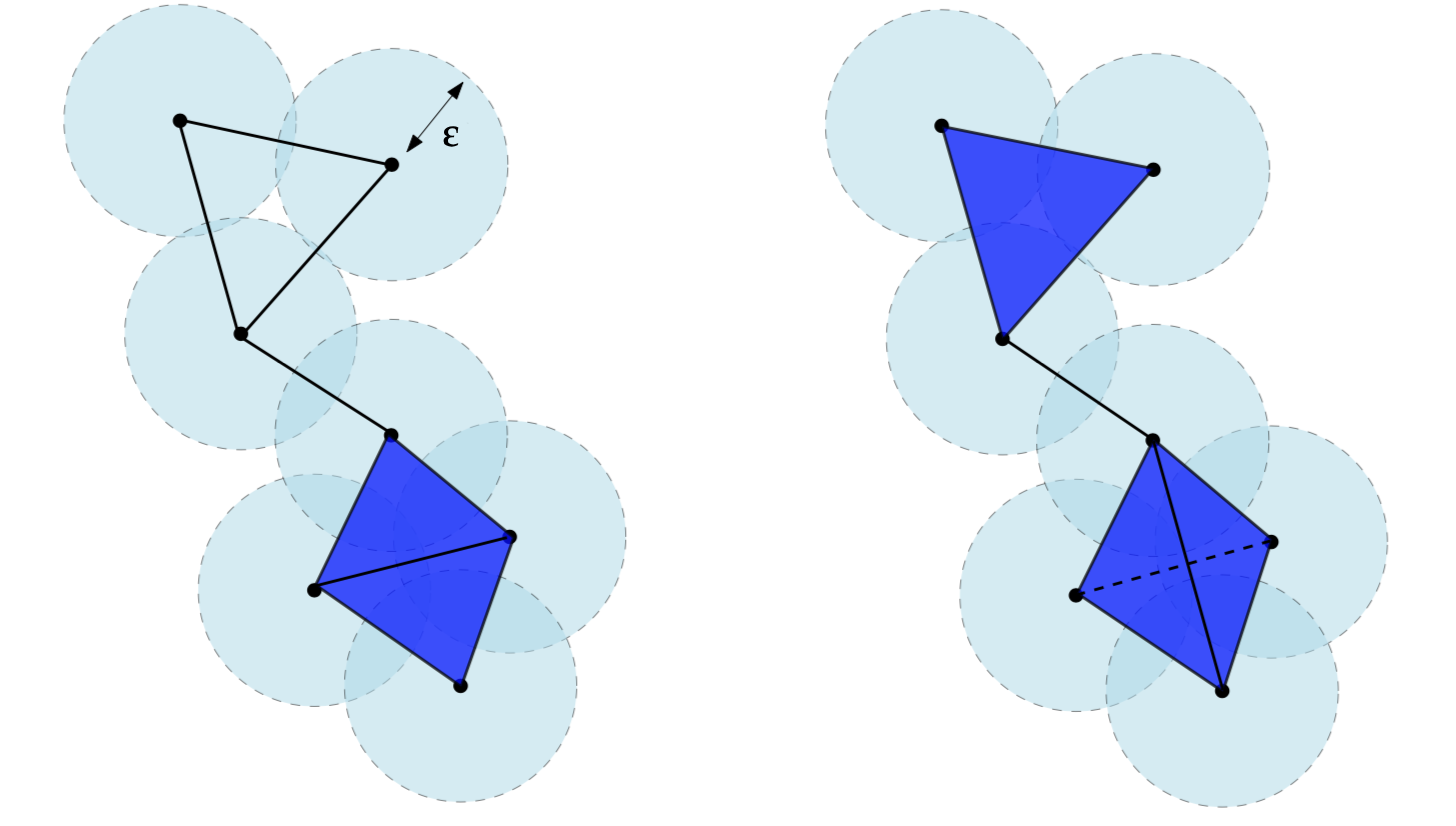
\includegraphics[width=110mm]{img/cech-vr.png}
	\caption{Representación de los complejos simpliciales \u Cech (izquierda) y Vietoris-Rips (derecha) para un conjunto de puntos en \( \mathbb{R}^2 \). En el complejo de \u Cech, los símplices se forman por la intersección no vacía de círculos de radio \(\varepsilon\) centrados en los puntos. El complejo de Vietoris-Rips conecta puntos que distan hasta \(2\varepsilon\), independientemente de las intersecciones de los círculos. Los símplices de mayor dimensión están coloreados en azul, resaltando las diferencias en la estructura simplicial generada por cada método. Fuente \cite{chazal2021introduction}.}
\end{figure}

El complejo de Vietoris-Rips es interesante en el estudio de complejos de \u Cech. Este hecho se debe a que estos últimos pueden ser aproximados por complejos de Vietoris-Rips:

\begin{proposicion}
	Sea \((X,d)\) un espacio métrico y sea \(V\) un subconjunto de puntos de \(X\). Entonces
	\[
		C(V, \varepsilon) \subseteq VR(V, 2\varepsilon) \subseteq C(V, 2\varepsilon).
	\]
\end{proposicion}
\begin{proof}
	La primera inclusión es inmediata pues si un punto \(x\) pertenece a la intersección \(\bigcap_{v \in V} B(v, \varepsilon)\), entonces la distancia para cada par de puntos de \(V\) es, a lo sumo, \(2 \varepsilon\). En consecuencia, cualquier símplice de \(C(V,\varepsilon)\) se encuentra en \(VR(V, 2\varepsilon)\).
	
	Para la segunda inclusión, consideremos ahora un símplice \(\sigma = \{v_0, \dots, v_p\}\) de \(VR(V, 2\varepsilon)\). Por la definición de complejo de Vietoris-Rips, tenemos que \(d(v_i, v_j) \leq 2\varepsilon\) para todo \(i,j \in \{0, \dots, p\}\). Considerando las bolas abiertas de radio \(2\varepsilon\) centradas en \(v_i\) y en \(v_j\), tenemos que su intersección es no vacía, pues \(v_i \in \overline{B}_{2\varepsilon}(v_j)\) y \(v_j \in \overline{B}_{2\varepsilon}(v_i)\). En el supuesto de que los puntos pertenecieran a la frontera de las bolas, la intersección de las bolas abiertas también sería no vacía pues \(\varepsilon > 0\). En consecuencia, tenemos que \(\sigma \in C(V,2\varepsilon)\).
\end{proof}

\section{Módulos de homología persistente}

El módulo de homología persistente es el objeto central de estudio en este capítulo. A partir de filtraciones de complejos simpliciales, esta estructura nos va a permitir realizar un estudio de la homología simplicial de dicha filtración.

\begin{definicion}
	Sea \(K\) un complejo simplicial. Una \textbf{filtración} \(\mathcal{F}\) de \(K\) es una familia totalmente ordenada de subcomplejos \(\{K^n\}_{n \in \N}\) tal que \(\emptyset, K \in \mathcal{F}\) y si \(i \leq j\), entonces \(K^i \subseteq K^j\). En particular, llamaremos a dicho orden \textbf{filtro}.
\end{definicion}
A partir de la definición anterior, podemos construir los complejos de cadenas asociados \(C(K^i;R)\) para todo \(i \in \N\). Así mismo, podemos obtener sus respectivos submódulos de ciclos \(Z_p(K^i)\) y bordes \(B_p(K^i)\) para cada $R$-módulo de cadenas orientadas \(C_p(K^i;R)\).
\begin{definicion}
	Sea \(\mathcal{F}\) una filtración, sea \(p\) un número natural y sean \(i,j \in \{0, \dots, n\}\) tales que $i \leq j$. Definimos el  \textbf{\((i,j)\)-ésimo \(R\)-módulo de homología persistente de dimensión \(p\)} asociado a \(\mathcal{F}\) como
	\[
		H_p^{i \to j}(\mathcal{F};R) := \im f_p^{i \to j},
	\]
	donde $f_p^{i \to j}$ es el homomorfismo inducido entre las clases de homología de la inclusión que va de $K^i$ a $K^j$. El rango de \(H_p^{i \to j}(\mathcal{F};R)\) diremos que es el \textbf{\((i,j)\)-ésimo número de Betti de persistencia de dimensión \(p\)} y lo notaremos por \(\beta_p^{i \to j}\).
\end{definicion}
\begin{proposicion}
	Sea \(\mathcal{F}\) una filtración del complejo simplicial \(K\). Entonces
	\[
		H_p^{i \to j}(\mathcal{F};R) \cong \frac{Z_p(K^i)}{B_p(K^j) \cap Z_p(K^i)}
	\]
	es un isomorfismo de \(R\)-módulos.
\end{proposicion}
\begin{proof}
	Sabemos que el cociente anterior está bien definido, pues \(Z_p(K^i) \cap B_p(K^j)\) es un submódulo de \(Z_p(K^i)\). Para ver que en efecto existe un isomorfismo, consideraremos la proyección \(\pi_i : Z_p(K^i) \to H_p(K^j;R)\). Aplicando el \nameref{teo:first-iso}, tenemos que 
	\[
		\frac{Z_p(K^i)}{\ker \pi_i} \cong \im \pi_i
	\]
	es un isomorfismo. Sin embargo, nótese que
	\begin{align*}
		\ker \pi_i &= \{z \in Z_p(K^i) : \pi_i(z) = [0] \}
				   = \{z \in Z_p(K^i) : [z] = [0] \} \\ 
				   &= \{z \in Z_p(K^i) : z \in B_p(K^j) \}
				   = B_p(K^j) \cap Z_p(K^i).
	\end{align*}
	Además, 
	\begin{align*}
		H_p^{i \to j}(\mathcal{F};R) &= \im f_p^{i \to j} = \{f_p^{i \to j}([z]) : [z] \in H_p(K^i;R) \} \\ 
							   &= \{[({i_{i,j}}_*)_p(z)] : z \in Z_p(K^i) \}  
							   = \{\pi_i(z) : z \in Z_p(K^i) \} 
							   = \im \pi_i.
	\end{align*}
\end{proof}
%
%\tikzset{every picture/.style={line width=0.75pt}} %set default line width to 0.75pt        
%
%\begin{tikzpicture}[x=0.75pt,y=0.75pt,yscale=-1,xscale=1]
%	%uncomment if require: \path (0,235); %set diagram left start at 0, and has height of 235
%	
%	%Shape: Ellipse [id:dp28793519162441483] 
%	\draw  [fill={rgb, 255:red, 74; green, 144; blue, 226 }  ,fill opacity=1 ] (81,72.52) .. controls (81,21.96) and (104.41,-19.03) .. (133.29,-19.03) .. controls (162.18,-19.03) and (185.59,21.96) .. (185.59,72.52) .. controls (185.59,123.08) and (162.18,164.07) .. (133.29,164.07) .. controls (104.41,164.07) and (81,123.08) .. (81,72.52) -- cycle ;
%	%Shape: Ellipse [id:dp5681689316325549] 
%	\draw  [fill={rgb, 255:red, 169; green, 208; blue, 255 }  ,fill opacity=1 ] (213.98,71.12) .. controls (213.98,20.55) and (237.39,-20.44) .. (266.27,-20.44) .. controls (295.15,-20.44) and (318.56,20.55) .. (318.56,71.12) .. controls (318.56,121.68) and (295.15,162.67) .. (266.27,162.67) .. controls (237.39,162.67) and (213.98,121.68) .. (213.98,71.12) -- cycle ;
%	%Shape: Ellipse [id:dp8309047921029127] 
%	\draw  [fill={rgb, 255:red, 169; green, 208; blue, 255 }  ,fill opacity=1 ] (349.94,72.52) .. controls (349.94,21.96) and (373.35,-19.03) .. (402.24,-19.03) .. controls (431.12,-19.03) and (454.53,21.96) .. (454.53,72.52) .. controls (454.53,123.08) and (431.12,164.07) .. (402.24,164.07) .. controls (373.35,164.07) and (349.94,123.08) .. (349.94,72.52) -- cycle ;
%	%Shape: Ellipse [id:dp6471754723664047] 
%	\draw  [fill={rgb, 255:red, 169; green, 208; blue, 255 }  ,fill opacity=1 ] (484.41,72.52) .. controls (484.41,21.96) and (507.82,-19.03) .. (536.71,-19.03) .. controls (565.59,-19.03) and (589,21.96) .. (589,72.52) .. controls (589,123.08) and (565.59,164.07) .. (536.71,164.07) .. controls (507.82,164.07) and (484.41,123.08) .. (484.41,72.52) -- cycle ;
%	%Shape: Ellipse [id:dp2887350161913229] 
%	\draw  [fill={rgb, 255:red, 74; green, 144; blue, 226 }  ,fill opacity=1 ] (226.68,99.38) .. controls (226.68,64.42) and (244.4,36.09) .. (266.27,36.09) .. controls (288.14,36.09) and (305.86,64.42) .. (305.86,99.38) .. controls (305.86,134.33) and (288.14,162.67) .. (266.27,162.67) .. controls (244.4,162.67) and (226.68,134.33) .. (226.68,99.38) -- cycle ;
%	%Shape: Ellipse [id:dp5997979826300346] 
%	\draw  [fill={rgb, 255:red, 74; green, 144; blue, 226 }  ,fill opacity=1 ] (362.64,100.78) .. controls (362.64,65.83) and (380.37,37.49) .. (402.24,37.49) .. controls (424.1,37.49) and (441.83,65.83) .. (441.83,100.78) .. controls (441.83,135.73) and (424.1,164.07) .. (402.24,164.07) .. controls (380.37,164.07) and (362.64,135.73) .. (362.64,100.78) -- cycle ;
%	%Shape: Ellipse [id:dp7175957985808079] 
%	\draw  [fill={rgb, 255:red, 74; green, 144; blue, 226 }  ,fill opacity=1 ] (505.7,114.81) .. controls (505.7,87.61) and (519.58,65.55) .. (536.71,65.55) .. controls (553.83,65.55) and (567.71,87.61) .. (567.71,114.81) .. controls (567.71,142.02) and (553.83,164.07) .. (536.71,164.07) .. controls (519.58,164.07) and (505.7,142.02) .. (505.7,114.81) -- cycle ;
%	%Straight Lines [id:da9382562350971808] 
%	\draw    (133.29,-19.03) -- (266.27,36.09) ;
%	%Straight Lines [id:da8538877694649378] 
%	\draw    (266.27,36.09) -- (402.24,37.49) ;
%	%Straight Lines [id:da415521229926751] 
%	\draw    (402.24,37.49) -- (536.71,65.55) ;
%	%Straight Lines [id:da5906511807851325] 
%	\draw [fill={rgb, 255:red, 74; green, 144; blue, 226 }  ,fill opacity=1 ] [dash pattern={on 0.84pt off 2.51pt}]  (266.27,16.65) -- (399.25,16.65) ;
%	%Straight Lines [id:da7445210416359846] 
%	\draw  [dash pattern={on 0.84pt off 2.51pt}]  (399.25,16.65) -- (536.71,114.81) ;
%	
%	% Text Node
%	\draw (260.27,-0.47) node [anchor=north west][inner sep=0.75pt]    {\(\alpha \)};
%	% Text Node
%	\draw (375.75,-4.04) node [anchor=north west][inner sep=0.75pt]    {\(f_{p}^{i,j-1}( \alpha )\)};
%	% Text Node
%	\draw (515.12,113.56) node [anchor=north west][inner sep=0.75pt]    {\(f_{p}^{i,j}( \alpha )\)};
%	% Text Node
%	\draw (100.29,-38.98) node [anchor=north west][inner sep=0.75pt]    {\(H_{p}( K_{i-1})\)};
%	% Text Node
%	\draw (242.52,-40.98) node [anchor=north west][inner sep=0.75pt]    {\(H_{p}( K_{i})\)};
%	% Text Node
%	\draw (370.99,-39.38) node [anchor=north west][inner sep=0.75pt]    {\(H_{p}( K_{j-1})\)};
%	% Text Node
%	\draw (510.2,-39.98) node [anchor=north west][inner sep=0.75pt]    {\(H_{p}( K_{j})\)};
%	% Text Node
%	\draw (260,12.4) node [anchor=north west][inner sep=0.75pt]    {\(\bullet \)};
%	% Text Node
%	\draw (393,12.4) node [anchor=north west][inner sep=0.75pt]    {\(\bullet \)};
%	% Text Node
%	\draw (528,108.4) node [anchor=north west][inner sep=0.75pt]    {\(\bullet \)};
%\end{tikzpicture}

La homología persistente facilita la interpretación de la homología en los distintos niveles de la filtración, permitiendo un análisis cuantitativo de su evolución. Al observar el nacimiento y desaparición de las clases de homología mediante los módulos de homología persistente, se obtiene información detallada de la estructura topológica general de la filtración.

\begin{definicion}
	Dada una filtración \(\mathcal{F}\), decimos que un elemento \(\alpha \neq 0\) en \(H_p(K^i;R)\) \textbf{nace} en \(K^i\) si \(\alpha \not\in H_{p}^{i-1 \to i}(\mathcal{F};R)\). Además, decimos que \(\alpha\) \textbf{muere} en \(K^j\) si se fusiona con una clase proveniente de una dimensión anterior cuando se desplaza de \(K^{j-1}\) a \(K^{j}\). Esto es, si \(f^{i \to j-1}_p(\alpha) \not\in H_{p}^{i-1 \to j-1}(\mathcal{F};R)\) pero \(f^{i \to j}_p(\alpha) \in H_{p}^{i-1 \to j}(\mathcal{F};R)\).
\end{definicion}

\section{Representación de la homología persistente}

Nuestro objetivo ahora es obtener una representación de la homología persistente que nos permita interpretarla. Originalmente, esta representación se ha realizado mediante los \textbf{diagramas de persistencia}. En estos diagramas, cada clase de homología que nace en un complejo simplicial \(K^{i}\) y muere en \(K^{j}\) se representa por un punto \((i, j)\) en el plano cartesiano, para cada dimensión \(p\).

Aunque intuitivos, los diagramas de persistencia presentan ciertas limitaciones. El principal problema radica en que no logran capturar de manera efectiva la multiplicidad de la persistencia; es decir, múltiples clases que nacen y mueren simultáneamente se representan mediante un mismo punto, lo que puede conducir a ambigüedades en la interpretación de los datos.

Para abordar estos problemas, Zomorodian y Carlsson introdujeron un enfoque innovador mediante el uso del \textbf{código de barras} \cite{zomorodian2004computing}. Este método no solo ofrece una visualización clara y detallada de la vida de cada clase de homología, sino que también facilita la interpretación de su multiplicidad y relevancia en el contexto de los datos analizados. Esta interpretación fue posible ya que demostraron que todo módulo de persistencia puede identificarse de manera biyectiva con una estructura algebraica más general, conocida como \textbf{módulos graduados}, bajo ciertas hipótesis.

A continuación profundizaremos en la aplicación y las implicaciones de estos métodos, explorando en detalle el Teorema de correspondencia como se discute en \cite{Corbet_2018}.

\begin{figure}
	\centering
	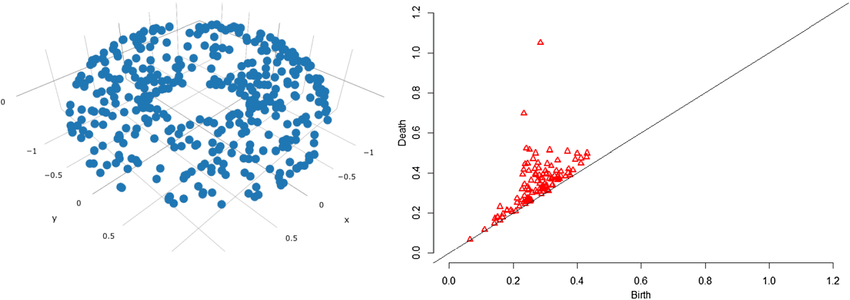
\includegraphics[width=\textwidth]{img/persistence-diagram.png}
	\caption{Diagrama de persistencia para la homología de dimensión 1 de la filtración de Vietoris-Rips de 2000 puntos i.i.d. en un toro. El gráfico destaca dos puntos significativos que representan las clases de equivalencia de los ciclos unidimensionales del toro, destacando su persistencia topológica. Fuente \cite{divol2019}.}
\end{figure}

\begin{definicion}
	Sea \( \mathcal{M} = \{\{M_i\}_{i \in \N}, \{f_{i,j}\}_{i \leq j \in \N}\} \) una familia de \( R \)-módulos. Diremos que dicha familia es un \textbf{módulo de persistencia discreto} sobre \( R \) si para cada \( i \leq j \) existe un homomorfismo de \( R \)-módulos \( f_{i,j}: M_i \to M_j \) tal que:
	\begin{enumerate}
		\item El homomorfismo \( f_i = f_{i,i} = \mathrm{id}_{M_i} \) para todo \( i \in \mathbb{N} \).
		\item La composición \( f_{i,k} \circ f_{i,j} = f_{i,k} \) para todo \( i \leq j \leq k \).
	\end{enumerate}
\end{definicion}
\begin{observacion}
	Nótese que con esta definición, todo módulo de homología persistente es de hecho un módulo de persistencia discreto. Dada una dimensión $p \in \Z$ fija, los $R$-módulos los componen los módulos de homología y sus homomorfismos inducidos por la inclusión cumplen dichas propiedades. 
\end{observacion}

\begin{definicion}
	Sean \(\mathcal{M} = \{\{M_i\}_{i \in \N}, \{f_{i,j}\}_{i \leq j \in \N}\}, \mathcal{N} = \{\{N_i\}_{i \in \N}, \{g_{i,j}\}_{i \leq j \in \N}\} \) dos módulos de persistencia discretos.  Diremos que la familia de homomorfismos \(\varphi_\bullet = \{\varphi_i\}_{i \in \N}\) tales que \(\varphi_i : M_i \to N_i\) es un \textbf{homomorfismo de módulos de persistencia discreto} si \(g_{i,j} \circ \varphi_i = \varphi_j \circ f_{i,j}\).
\end{definicion}
La anterior definición es equivalente a decir que el diagrama
\[
	\xymatrix{
		M_0 \ar@{->}[r]^{f_0} \ar@{->}[d]^{\varphi_0} & M_1 \ar@{->}[r]^{f_1} \ar@{->}[d]^{\varphi_1} & \cdots \ar@{->}[r]^{f_{i-1}} & M_i \ar@{->}[r]^{f_i} \ar@{->}[d]^{\varphi_i} & M_{i+1} \ar@{->}[r]^{f_{i+1}} \ar@{->}[d]^{\varphi_{i+1}} & \cdots \\
		N_0 \ar@{->}[r]^{g_0} & N_1 \ar@{->}[r]^{g_1} & \cdots \ar@{->}[r]^{g_{i-1}} & N_i \ar@{->}[r]^{g_i} & N_{i+1} \ar@{->}[r]^{g_{i+1}} & \cdots
	}
\]
conmuta. En las condiciones anteriores, los módulos de persistencia discretos junto a sus homomorfismos forman una categoría que notaremos por \(R\)-\(\Cat{PersMod}\). Claramente se tiene que existe el homomorfismo identidad $\id_\mathcal{M} : \mathcal{M} \to \mathcal{M}$, donde a cada módulo y homomorfismo de módulos se le asocia él mismo. Además, la identidad conmuta con la familia de homomorfismos de módulos, pues es la composición con la identidad de homomorfismos de módulos componente a componente. Veamos ahora la asociatividad en la composición de los homomorfismos de módulos de persistencia discretos. Consideremos cuatro módulos de persistencia discretos $\mathcal{M} = \{\{M_i\}_{i \in \mathbb{N}}, \{f_{i,j}\}_{i \leq j \in \mathbb{N}}\}$,
$\mathcal{N} = \{\{N_i\}_{i \in \mathbb{N}}, \{g_{i,j}\}_{i \leq j \in \mathbb{N}}\}$,
$\mathcal{P} = \{\{P_i\}_{i \in \mathbb{N}}, \{h_{i,j}\}_{i \leq j \in \mathbb{N}}\}$ y
$\mathcal{Q} = \{\{Q_i\}_{i \in \mathbb{N}}, \{p_{i,j}\}_{i leq j \in \mathbb{N}}\}$; y tres homomorfismos \(\varphi_\bullet : \mathcal{M} \to \mathcal{N}\), \(\psi_\bullet : \mathcal{N} \to \mathcal{P}\), y \(\theta_\bullet : \mathcal{P} \to \mathcal{Q}\). Para demostrar la asociatividad, necesitamos verificar que
\[
(\theta \circ (\psi \circ \varphi))_i = ((\theta \circ \psi) \circ \varphi)_i \quad \forall i \in \mathbb{N}.
\]
Sin embargo, dicha composición es la asociatividad de la composición de homomorfismos de módulos componente a componente, por lo que tenemos que:
\[
\theta_i \circ (\psi_i \circ \varphi_i) = (\theta_i \circ \psi_i) \circ \varphi_i.
\]

Además, para cualquier \(i \leq j\) en \(\mathbb{N}\), necesitamos mostrar que:
\[
h_{i,j} \circ (\theta \circ (\psi \circ \varphi))_i = (\theta \circ (\psi \circ \varphi))_j \circ f_{i,j}.
\]
Sustituyendo la definición de composición, esto se reduce a verificar que
\[
h_{i,j} \circ (\theta_i \circ (\psi_i \circ \varphi_i)) = (\theta_j \circ (\psi_j \circ \varphi_j)) \circ f_{i,j} \quad  i \leq j \text{ en } \N.
\]
O equivalentemente, que $((h_{i,j} \circ \theta_i) \circ \psi_i) \circ \varphi_i = \theta_j \circ (\psi_j \circ (\varphi_j \circ f_{i,j}))$.
Debido a que cada homomorfismo respeta las estructuras de los módulos de persistencia, tenemos:
\[
h_{i,j} \circ \theta_i = \theta_j \circ p_{i,j},
\]
\[
p_{i,j} \circ \psi_i = \psi_j \circ g_{i,j},
\]
\[
g_{i,j} \circ \varphi_i = \varphi_j \circ f_{i,j}.
\]
Aplicando estas igualdades y la asociatividad de homomorfismos de módulos, concluimos que:
\begin{align*}
h_{i,j} \circ (\theta_i \circ (\psi_i \circ \varphi_i)) &= ((h_{i,j} \circ \theta_i) \circ \psi_i) \circ \varphi_i = ((\theta_j \circ p_{i,j}) \circ \psi_i) \circ \varphi_i \\
&= (\theta_j \circ (p_{i,j} \circ \psi_i)) \circ \varphi_i = (\theta_j \circ (\psi_j \circ g_{i,j})) \circ \varphi_i \\
&= \theta_j \circ ((\psi_j \circ g_{i,j}) \circ \varphi_i) = \theta_j \circ (\psi_j \circ (g_{i,j} \circ \varphi_i))
= \theta_j \circ (\psi_j \circ (\varphi_j \circ f_{i,j})).
\end{align*}

\begin{definicion}
	Sea \( R \) un anillo. Diremos que \( R \) es un \textbf{anillo graduado} si puede descomponerse como una suma directa
	\[
	R = \bigoplus_{n=0}^{\infty} R_n,
	\]
	donde \( R_m R_n \subseteq R_{m+n} \) para todos \( m, n \in \mathbb{Z} \). Los elementos de \( R_n \) distintos de cero se denominan \textbf{homogéneos de grado \( n \)}.
\end{definicion}

\begin{definicion}
	Sea \( R \) un anillo graduado y sea \( M \) un \( R \)-módulo. Diremos que \( M \) es un \textbf{módulo graduado} si puede escribirse como
	\[
	M = \bigoplus_{n=0}^{\infty} M_n,
	\]
	donde \( M_n \) son grupos abelianos y \( R_m M_n \subseteq M_{m+n} \) para todos \( m, n \in \mathbb{Z} \). Un elemento de \( M_n \) distinto de cero se llama \textbf{homogéneo de grado \( n \)}.
\end{definicion}

Los módulos graduados no son más que un tipo particular de módulos. Para cada módulo graduado \( M \), el morfismo identidad \( \mathrm{id}_M : M \to M \) es simplemente el morfismo identidad de $R$-módulos. Este morfismo es claramente un homomorfismo de módulos graduados que preserva la graduación. Consideremos ahora dos módulos graduados \( M \), \( N \) y un homomorfismo de módulos graduados \( f: M \to N \). Si tenemos otro módulo graduado \( P \) y un homomorfismo \( g: N \to P \), su composición \( g \circ f \) es la composición de homomorfismos de $R$-módulos. Por lo tanto, la asociatividad de la composición se sigue directamente de la asociatividad de la composición de homomorfismos de $R$-módulos. En consecuencia, los módulos graduados sobre \( R \) junto con los homomorfismos de módulos graduados forman una categoría, que denotaremos por \( R\text{-}\mathbf{GrMod} \).

Los módulos de persistencia discretos sobre un anillo \(R\) y los \(R[t]\)-módulos graduados son conceptos íntimamente relacionados. Si \(\mathcal{M}\) es un módulo de persistencia discreto, podemos definir un \(R[t]\)-módulo graduado \(\alpha(\mathcal{M})\) como
\[
	\alpha(\mathcal{M}) = \bigoplus_{i \in \N} M_i,
\]
donde el producto por \(t\) lo definimos como \(t \cdot m_i = f_{i,i+1}(m_i)\) para todo \(m_i \in M_i\). Análogamente, podemos definir un módulo de persistencia discreto a partir de un \(R[t]\)-módulo \(\bigoplus_{i \in \N} M_i\), de forma que
\[
	\beta \left( \bigoplus_{i \in \N} M_i \right) = \mathcal{M}.
\]
Aquí, los morfismos los obtenemos a partir del producto por \(t\), esto es, \(f_{i, i+1}(m_i) = t \cdot m_i\) para todo \(m_i \in M_i\). El siguiente resultado nos proporciona formalmente cómo de íntima 
es esta relación.

\begin{lema}
	\label{lem:repr-carlsson-no-finito}
	Las aplicaciones \(\alpha\) y \(\beta\) definidas anteriormente forman una pareja isomorfa de funtores covariantes entre \(R\)-\(\Cat{PersMod}\) y \(R[t]\)-\(\Cat{GrMod}\). En particular, ambas categorías son isomorfas.
\end{lema}
\begin{proof}
	Sea \(\varphi_\bullet : \mathcal{M} \to \mathcal{N}\) un morfismo de módulos de persistencia discretos. Definamos
	\[
		\alpha(\varphi_{\bullet}) : \bigoplus_{i \in \N} M_i \to \bigoplus_{i \in \N} N_i
	\]
	donde a cada \(m_i \in M_i\) le asignamos \(\varphi_i(m_i)\) para cada \(i \in \N\). Veamos que \(\alpha : R\)-\(\Cat{PersMod} \to R[t]\)-\(\Cat{GrMod}\) es un funtor covariante. Primero veamos que \(\alpha(\varphi_{\bullet})\) es un morfismo de módulos graduados. Tenemos que \(\alpha(\varphi_{\bullet})\) es un homomorfismo de grupos pues cada \(\varphi_{i}\) lo es, cumple que \(\alpha(\varphi_{i})(M_i) \subseteq N_i\) y además, si \(m = (m_0, m_1, \ldots)\) es un elemento de \(\mathcal{M}\), entonces
	\begin{align*}
		\alpha(\varphi_{\bullet})(tm) &= \alpha(\varphi_{\bullet})(0, tm_0, tm_1, \ldots) = (0, \varphi_0(tm_0), \varphi_1(tm_1), \ldots) \\
		&= (0, t\varphi_0(m_0), t\varphi_1(m_1), \ldots) = t\alpha(\varphi_{\bullet})(m),
	\end{align*}
	donde la última igualdad es consecuencia de la segunda propiedad de los morfismos de módulos de persistencia discretos. 
	En cuanto a las propiedades funtoriales, es evidente que \(\alpha\) lleva identidades en identidades. Además, si \(\psi_\bullet\) es otro morfismo de módulos de persistencia discretos, tenemos que
	\begin{align*}
		(\alpha(\psi_\bullet \circ \varphi_\bullet))(m) = (\psi_i(\varphi_i(m_i)))_{i \in \N} = \alpha (\psi_\bullet)(\varphi_i(m_i))_{i \in \N} = (\alpha(\psi_\bullet) \circ \alpha(\varphi_\bullet))(m).
	\end{align*}
	
	Consideremos ahora el homomorfismo de \(R[t]\)-módulos graduados
	\[
		\eta : \bigoplus_{i \in \N} M_i \to \bigoplus_{i \in \N} N_i,
	\]
	que para cada \(i \in \N\) induce un homomorfismo \(\eta_i : M_i \to N_i\) compatible con el producto por \(t\). En consecuencia, el diagrama
	\[
	\xymatrix{
		M_0 \ar@{->}[r]^{t} \ar@{->}[d]^{\eta_0} & M_1 \ar@{->}[r]^{t} \ar@{->}[d]^{\eta_1} & \cdots \ar@{->}[r]^{t} & M_i \ar@{->}[r]^{t} \ar@{->}[d]^{\eta_i} & M_{i+1} \ar@{->}[r]^{t} \ar@{->}[d]^{\eta_{i+1}} & \cdots \\
		N_0 \ar@{->}[r]^{t} & N_1 \ar@{->}[r]^{t} & \cdots \ar@{->}[r]^{t} & N_i \ar@{->}[r]^{t} & N_{i+1} \ar@{->}[r]^{t} & \cdots
	}
	\]
	es conmutativo. Definamos ahora \(\beta(\eta) = (\eta_0, \eta_1, \ldots)\) y veamos que es un homomorfismo de módulos de persistencia discretos entre \(\mathcal{M}\) y \(\mathcal{N}\). En consecuencia, \(\beta\) nos da homomorfismos de grupos \(\eta_i : M_i \to N_i\) que, a su vez, son homomorfismos de \(R\)-módulos. Para comprobarlo, basta tomar cualquier \(r \in R\) y \(m_i \in M_i\) y vemos que \(\eta_i(rm_i) = \eta(rm_i) = r \eta(m_i) = r \eta_i(m_i)\). Como los homomorfismos de \(R\)-módulos de \(\mathcal{M}\) y \(\mathcal{N}\) se obtienen mediante la multiplicación por \(t\), entonces para todo \(m_i \in M_i\) tenemos que
	\[
		\eta_{i+1}(tm_i) = \eta(tm_i) = t\eta(m_i) = t \eta_i(m_i),
	\]
	por lo que \(\beta(\eta)\) es un homomorfismo de módulos de persistencia discretos.
	Claramente \(\beta\) conserva la identidad. Luego para otro \(\theta : \mathcal{M} \to \mathcal{N}\) y cualquier \(m=(m_i)_{i \in \N} \in \mathcal{M}\),
	\[
		(\beta(\theta \circ \eta))(m) = (\theta(\eta(m_i)))_{i \in \N} = \beta(\theta)(\eta(m_i))_{i \in \N} = (\beta(\theta) \circ \beta(\eta))(m).
	\]
	Esto es, \(\beta\) es un funtor covariante. Finalmente, por la construcción de \(\alpha\) y \(\beta\) tenemos que \(\beta \circ \alpha\) es el funtor identidad en \(R[t]\)-\(\Cat{GrMod}\) y que \(\alpha \circ \beta\) es el funtor identidad en \(R\)-\(\Cat{PersMod}\).
\end{proof}

En la práctica generalmente trabajaremos con módulos de persistencia que cumplen ciertas condiciones de finitud. Por ello, resulta de gran interés conocer si la correspondencia recién realizada se sigue cumpliendo bajo estos casos.

\begin{definicion}
	Diremos que un módulo de persistencia discreto \(\mathcal{M}\) es de \textbf{tipo finito} si existe \(N \in \N\) de forma que para todo \(i,j \in \N\) tal que \(N \leq i \leq j\) el homomorfismo \(f_{i,j}\) es un isomorfismo.
\end{definicion}

\begin{definicion}
	Diremos que un módulo de persistencia discreto \(\mathcal{M}\) es de \textbf{tipo finitamente presentado (generado)} si es de tipo finito y además, \(M_i\) es finitamente presentado (generado) para todo \(i \in \N\).
\end{definicion}

Nuestro objetivo será probar que el \autoref{lem:repr-carlsson-no-finito} sigue siendo cierto para los módulos de persistencia discretos de tipo finitamente presentados.

\begin{lema}
	\label{lem:alpha-finito-presentado}
	Sea \(\mathcal{M}\) un módulo de persistencia discreto. Si \(\mathcal{M}\) es de tipo finitamente presentado, entonces \(\alpha(\mathcal{M})\) es finitamente presentado.
\end{lema}
\begin{proof}
	Consideremos \(N \in \N\) de forma que \(f_{i,j} : M_i \to N_i\) es un isomorfismo para todo \(N \leq i \leq j\). Sea \(G\) un conjunto de generadores de \(M_i\). Queremos ver que \(G = \bigcup_{i=1}^N G_i\) es un sistema de generadores también para \(\alpha(\mathcal{M})\). Para ello, veamos que todo elemento homogéneo de \(\alpha(\mathcal{M})\) está generado por la unión de los \(G_i\). Fijemos \(k \in \N\) y sea \(m_k \in \alpha(\mathcal{M})\) un elemento homogéneo de grado \(k\). Si \(k \leq N\), entonces \(m_k\) está generado por los elementos de \(G_k\) por construcción. Si \(k > N\), veamos que \(m_k\) está generado por \(G_N\). Por ser \(f_{N,k}\) un isomorfismo, podemos tomar \(m_N = f^{-1}_{N,k}(m_k)\). Pero como \(m_D\) está generado por \(G_N\), entonces \(m_k\) está generado por \(f_{N,k}(G_N)\). Por como hemos construido \(\alpha\), \(f_{N,k}(G_N) = t^{k-N}G_N\) y como \(t^{k-N} \in R[t]\), entonces \(m_k\) está generado por \(G_N\). En consecuencia, \(\alpha(\mathcal{M})\) es finitamente generado.
	
	Para ver que \(\alpha(\mathcal{M})\) es finitamente presentado, consideremos el epimorfismo \(\mu_i : R^{n_i} \to M_i\) que genera \(M_i\) por extensión lineal sobre \(G_i\). Considerando \(n = \sum_{i=1}^N n_i\), existe una aplicación \(\mu : R[t]^N \to \alpha(\mathcal{M})\) que corresponde al sistema de generadores \(G\). Para cada \(g_i \in G\), denotemos por \(e_i\) a su correspondiente elemento en el sistema de generadores de \(R[t]^N\).
	
	A continuación definamos un conjunto finito de elementos del núcleo de \(\mu\). sea \(H_i\) el sistema de generadores de \(\ker \mu_i\) para cada \(0 \leq i \leq N\). Es claro que \(H_i \subseteq \ker \mu_i\). Es más, para cualquier \(0 \leq i < j \leq N\) y cualquier \(g_i \in G_i\) tal que \(f_{i,j}(g_i) \neq 0\), tenemos que 
	\[
		f_{i,j}(g_i) = \sum_{k=0}^{n_j} \lambda_k {g_j}_k
	\]
	donde \(\lambda_k \in R\) y \(G_i = \{ {g_j}_0, {g_j}_1, \ldots, {g_j}_k \}\). Por tanto, el correspondiente elemento 
	\[
		t^{j-i}e_i - \sum_{k=0}^{n_j} \lambda_k {e_j}_k
	\]
	pertenece al \(\ker \mu\). Denotemos ahora por \(H_{i,j}\) al conjunto finito obtenido tomando los elementos de la forma de la expresión anterior para cada \(g_i \in G_i\) tal que \(f_{i,j}(g_i) \neq 0\). Sea \(H = \bigcup_{i=0}^N H_i \cup \bigcup_{0 < i \leq j \leq N} H_{i,j}\).
	
	A continuación, fijemos un elemento \(x\) del núcleo de \(\mu\) de la forma
	\[
		x = \sum_l \lambda_l e_l
	\] de forma que \(\lambda_l \in R[t]\) y \(e_l\) es un generador de \(R[t]^n\). Podemos suponer sin pérdida de generalidad que \(x\) es homogéneo de algún grado \(k\). Veamos por casos que \(x\) es finitamente generado por los elementos de \(H_k\).
	
	Supongamos que \(k \leq N\) y que todos los escalares \(\lambda_l\) son de grado \(0\). Entonces, todos los \(e_l\) que aparecen en \(x\) son del mismo grado y por tanto, sus imágenes por \(\mu\) son generadores de \(M_k\). Es decir, \(x\) está generado por \(H_k\).
	
	Supongamos ahora qe \(k \leq N\) y que algún \(\lambda_l\) es de grado positivo. Por ser \(x\) homogéneo, entonces \(\lambda_l\) es de la forma \(r_l t^{d_l}\), donde \(r_l \in R\) y \(d_l > 0\). Como el grado de \(e_l\) es \(k - d_l\), entonces existe un elemento \(h_l \in H_{k-d_l,k}\) de la forma 
	\[
		h_l = t^{d_l}e_l - \sum_{m=0}^{n_l} \tilde{\lambda}_m {e_l}_m,
	\]
	donde todos los \({e_l}_m\) son de grado \(k\) y \(\tilde{\lambda}_m \in R\). Por consiguiente, en \(x - r_l h_l\) el coeficiente de \(e_l\) en \(x\) es \(0\) en \(t\) y por tanto, sólo estamos introduciendo sumandos de grado \(0\) en \(t\).
	
	Iterando esta construcción para cada sumando de con coeficiente de grado positivo, obtenemos un elemento \(x' = x - \sum_w r_w h_w\), donde \(r_w \in R\), \(h_w \in H\) y \(x'\) tiene solamente coeficientes de grado \(0\) en \(t\). Esto es, \(x = x' \sum_w r_w h_w\). Finalmente, aplicando la primera parte de la demostración tenemos que \(x\) es generado por \(H\).
	
	Para concluir, consideremos \(k > N\). En dicho caso, cada \(\lambda_l\) es de grado al menos \(k - N\), pues el grado maximal de \(e_l\) es \(N\). Luego \(x = t^{k-N}x'\), donde \(x'\) es homogéneo de grado \(N\). Como \(0 = \mu(x) = t^{k-N} \mu(x')\), entonces \(x' \in \ker \mu\). Por la segunda parte de la demostración, concluimos que \(x'\) es generado por \(H\) y por tanto, \(x\) también.
\end{proof}

Para los siguientes dos lemas, fijaremos el \(R[t]\)-módulo graduado finitamente presentado \(\mathbf{M} = \oplus_{i \in \N} M_i\) junto con la aplicación \(\mu : R[t]^n \to \mathbf{M}\) cuyo núcleo es finitamente generado. Consideremos además el sistema de generadores \(G = \{g_1, \ldots, g_n\}\) de \(\mathbf{M}\) y sea \(H = \{h_1, \ldots, h_m\}\) un sistema de generadores de \(\ker \mu\). Además, consideremos que tanto los elementos de \(G\) como de \(H\) son homogéneos del grado del respectivo módulo. Finalmente, vamos a asumir que dichos elementos están ordenados por grado en orden no decreciente.

\begin{lema}
	\label{lem:finit-pres}
	Cada \(M_i\) de \(\mathbf{M}\) es finitamente presentado como un \(R\)-módulo.
\end{lema}
\begin{proof}
	Veamos primero que \(M_i\) es finitamente generado. Sea \(d_j\) el grado de \(g_j\) para \(1 \leq j \leq n\). Sea \(n_i\) el número de elementos de \(G\) con grado menor o igual que \(i\). Definamos \(\mu_i : R^{n_i} \to M_i\) de forma que \(\mu_i\) asigne al \(j\)-ésimo generador \({e_i}_j \in R^{n_i}\) el elemento \(t^{i-d_j}g_j\). Cada elemento \(x \in M_i\) es un componente homogéneo de grado \(i\) de una combinación lineal de los generadores de \(\mathbf{M}\). Dado que solo los generadores \(g_j\) cuyo grado \(d_j\) es menor o igual que \(i\) pueden contribuir a esta combinación para formar un elemento de grado \(i\), \(x\) puede expresarse como:
	\[
	x = \sum_{d_j = 1}^i r_j t^{i-d_j} g_j,
	\]
	donde \(r_j \in R\). Considerando el generador en \(R^{n_i}\) cuyas entradas son los coeficientes \(r_j\), entonces
	\[
	\mu_i((r_1, \ldots, r_{n_i})) = \sum_{d_j = 1}^i r_j t^{i-d_j} g_j = x
	\]
	y en consecuencia, $\mu_i$ es sobreyectivo. Esto es, \(M_i\) es finitamente generado.
	
	A continuación veamos que \(\ker \mu_i\) también es finitamente generado. Sean \(e_1, \ldots, e_n\) los generadores de \(R[t]^n\) con imagen \(g_1, \ldots, g_n\) por \(\mu\) respectivamente. Sea \(m_i\) el número de elementos \(h_j\) de \(H\) cuyo grado \(d'_j\) es menor o igual que \(i\). Para cada \(h_j\) tal que \(1 \leq j \leq m_i\), consideremos \(t^{i-d'_j} h_j\) que podemos reescribir como
	\[
		t^{i-d'_j} h_j = \sum_{k=1}^{m_i} r_k t^{i-d_k} e_k
	\]
	para ciertos \(r_k \in R\). Definamos ahora 
	\[
		{h_j}_i = \sum_{k=1}^{n_i} r_k {e_k}_i
	\]
	y definamos \(H_i = \{ {h_j}_i : 1 \leq i \leq m_i \}\). Veamos que \(H_i\) genera el núcleo de \(\mu\). Es claro que \(\mu_i({h_j}_i) = \mu(h_j) = 0\). Fijemos ahora un elemento arbitrario \(x\) de \(\ker \mu_i\). Tenemos entonces que \(x\) es combinación lineal de \(\{{e_1}_i, \ldots, {e_{n_i}}_i\}\) con coeficientes en \(R\). Reemplazando \({e_j}_i\) por \(t^{i-d_j}e_j\), obtenemos un elemento homogéneo \(x' \in R[t]^n\) de grado \(i\). Por hipótesis, podemos escribir \(x'\) como combinación de elementos de \(H\) de forma que
	\[
		x' = \sum_{k=1}^{m_i} r'_k t^{i-d'_k} {h_k}_i
	\]
	donde \(r'_k \in R\). En consecuencia, veamos que
	\[
		x = \sum_{k=1}^{m_i} r'_k {h_k}_i.
	\]
	Para ello, procederemos comparando coeficientes. Consideremos \(j \in \{1, \ldots, n_i\}\) y sea \(c_j \in R\) el coeficiente de \({e_j}_i\) en \(x\). Sea \(c'_j\) el coeficiente de \({e_j}_i\) en la suma de la expresión anterior, escribiendo cada \({h_k}_i\) como combinación lineal de los \({e_j}_i\). Por la construcción realizada, \(c_j\) es el coeficiente de \(t^{i-d_j} e_j\) en \(x'\) y \(c'_j\) es el coeficiente de \(t^{i-d_j} e_j\) en la suma \(\sum_{k=1}^{m_i} r'_k t^{i-d'_k} {h_k}_i\). Esto es, \(c_j = c'_j\). Como \(x\) se escogió de manera arbitraria de \(\ker \mu_i\), entonces \(H_i\) lo genera.
\end{proof}

\begin{lema}
	\label{lem:beta-finito-presentado}
	\(\beta(\mathbf{M})\) es de tipo finito. En particular, es de tipo finitamente presentado.
\end{lema}
\begin{proof}
	Sea \(N\) el grado máximo de los \(g_j \in G_j\), \(h_k \in H_k\) de forma que \(1 \leq j \leq n\), \(1 \leq k \leq m\). Veamos que la multiplicación por \(t\) induce un isomorfismo entre \(M_i\) y \(M_{i+1}\) para todo \(i \geq N\).
	
	Si \(y \in M_{i+1}\), entonces existen \(\lambda_j \in R[t]\) de grado al menos \(1\) de forma que \(y = \sum_{j=1}^n \lambda_j g_j\). Por tanto, \(y = ty'\) donde \(y' \in M_i\) mostrando que la multiplicación por \(t\) es sobreyectiva.
	
	Para ver que es inyectiva, consideremos \(y \in M_i\) de forma que \(ty = 0\). Sea \(x \in R[t]^n\) tal que \(\mu(x) = y\). Entonces \(\mu(tx) = ty = 0\) y por tanto, veamos \(tx\) se puede escribir como
	\[
		tx = \sum_{j=0}^m \tilde{\lambda}_j h_j,
	\]
	donde cada \(\lambda_j\) no trivial es un polinomio de grado al menos \(1\). Es inmediato, pues cada \(h_j\) es de grado menor o igual que \(N\) y \(tx\) es de grado mayor o igual que \(N+1\). En consecuencia, también podemos descomponer \(tx\) como
	\[
		tx = \sum_{j=0}^m t \lambda_j h_j = t \sum_{j=0}^m \lambda_j h_j.
	\]
	Por ser \(R[t]^n\) un módulo libre, tenemos que \( x = \sum_{j=0}^m \lambda_j h_j\) y por tanto, \(x \in \ker \mu\) lo que implica que \(y = 0\).
\end{proof}

\begin{teorema}[Teorema de correspondencia]
	\label{teo:correspondence}
	Sea \( R \) un anillo unitario. Entonces, un isomorfismo entre la categoría de \(R[t]\)-módulos graduados finitamente presentados y la categoría de módulos de persistencia discretos.
\end{teorema}
\begin{proof}
	Estas categorías son subcategorías de \(R[t]\)-\(\Cat{GrMod}\) y \(R\)-\(\Cat{PersMod}\) respectivamente. Restringiendo \(\alpha\) y \(\beta\) a dichas subcategorías, por el \autoref{lem:alpha-finito-presentado} tenemos qe \(\alpha\) es un funtor covariante de los módulos de persistencia discretos de tipo finitamente presentados a los \(R[t]\)-módulos graduados finitamente presentados. Así mismo, por los lemas \ref{lem:finit-pres} y \ref{lem:beta-finito-presentado}, \(\beta\) es un funtor covariante de los \(R[t]\)-módulos graduados finitamente presentados a los módulos de persistencia discretos de tipo finitamente presentados. En consecuencia, estas subcategorías son isomorfas.
\end{proof}

El Teorema de descomposición de módulos graduados nos dará la clave para representar los módulos de persistencia.

\begin{teorema}[Teorema de descomposición de módulos graduados]
	\label{teo:desc-mod-grad}
	Sea $F$ un cuerpo y sea \( M \) un \( F[t] \)-módulo graduado finitamente generado. Entonces \( M \) se descompone de manera única, salvo isomorfismos, como
	\[
	M \cong \left( \bigoplus_{i=1}^{n-m} t^{a_i} \cdot R[t] \right) \oplus \left( \bigoplus_{j=1}^{m} t^{b_j} \cdot \frac{R[t]}{\langle t^{c_j} \rangle} \right),
	\]
	donde \( a_i, b_j, c_j \in \mathbb{N} \), y para cada \( j \), \( t^{c_j} \) es un elemento homogéneo tal que divide a \( t^{c_{j+1}} \).
\end{teorema}
\begin{proof}
	Véase \cite{webb1985decomposition}.
\end{proof}

De manera intuitiva, primero hemos construido una única estructura algebraica que contiene todos los complejos de la filtración. Después, hemos seguido calculando una suma directa a partir de los complejos, llegando así a un espacio mucho más grande que está graduado según el orden inducido de la filtración. A continuación, recordamos el momento en que cada símplice entra utilizando un coeficiente polinomial, codificando así el orden de filtración en el anillo de coeficientes polinomiales. A partir de aquí, el \nameref{teo:desc-mod-grad} nos proporciona una factorización simple cuando el anillo base es un cuerpo \( F \). Aquí, el anillo graduado \( F[t] \) es un DIP y sus únicos ideales graduados son homogéneos de la forma \( \langle t^n \rangle = t^n \cdot R[t] \), donde \( n \geq 0 \). Ahora que hemos transformado los módulos de persistencia discretos en objetos más manejables, queremos parametrizar las clases de isomorfismo de los \( F[t] \)-módulos por objetos más sencillos de interpretar.

\begin{definicion}
	Definimos un \textbf{$\mathcal{P}$-intervalo} como un par ordenado \( (i, j) \) tal que \( 0 \leq i \leq j \leq \mathbb{Z}^{\infty} = \mathbb{Z} \cup \{+\infty\} \).
\end{definicion}

Nuestro objetivo ahora es asociar un \( F[t] \)-módulo graduado a un conjunto \( S \) de $\mathcal{P}$-intervalos mediante una biyección \( Q \). Para ello, definimos \( Q(i, j) = t^i F[t]/\langle t^{j-i}\rangle \) para el $\mathcal{P}$-intervalo \( (i, j) \). Es claro que \( Q(i, +\infty) = t^i F[t] \). Además, para un conjunto de $\mathcal{P}$-intervalos \( S = \{(i_1, j_1), (i_2, j_2), \ldots, (i_n, j_n)\} \), definimos
\[
Q(S) = \bigoplus_{l=1}^n Q(i_l, j_l).
\]
Nuestra correspondencia puede ahora redefinirse como sigue.

\begin{corolario}
La correspondencia \( S \mapsto Q(S) \) define una biyección entre los conjuntos finitos de $\mathcal{P}$-intervalos y los módulos graduados finitamente generados sobre el anillo graduado \( F[t] \). Consecuentemente, las clases de isomorfismo de los módulos de persistencia de tipo finito sobre \( F \) están en correspondencia biyectiva con los conjuntos finitos de $\mathcal{P}$-intervalos.
\end{corolario}

En el contexto de filtraciones de complejos simpliciales, este resultado da lugar a la descripción de la homología persistente conocida como \textbf{código de barras}: cada $\mathcal{P}$-intervalo $(i, j)$ describe un ciclo que aparece en la filtración $i$ y especifica su clase de homología hasta que se convierte en borde en el instante $j$. Finalmente, condensamos el desarrollo realizado en el siguiente corolario: 

\begin{figure}
	\label{fig:barcode}
	\centering
\begin{tikzpicture}[scale=3]
	% Vertical dashed lines
	\draw[dashed, lightgray] (0,0) -- (0,.8);
	\draw[dashed, lightgray] (1,0) -- (1,.8);
	\draw[dashed, lightgray] ({sqrt(3)},0) -- ({sqrt(3)},.9);
	\draw[dashed, lightgray] (2,0) -- (2,.9);
	% Axis
	\draw [-latex,shorten >=-3pt] (-.2,0) -- (3,0) node [below] {\(\phantom{\sqrt{3}}t\phantom{\sqrt{3}}\)};
	\foreach \x in  {0,1,2}
	\node at (\x,0) {\(\bullet\)}
	node at (\x,0) [below] {\(\phantom{\sqrt{3}}\x\phantom{\sqrt{3}}\)};
	\node at ({sqrt(3)},0) {\(\bullet\)}
	node at ({sqrt(3)},0) [below] {\(\sqrt{3}\)};
	% Horizontal lines
	\draw [{*[fill=white]}-,shorten <=-2.4pt] (0,.2) -- (3,.2);
	\foreach \x in  {.3,.4,...,.7}
	\draw [{*[fill=white]}-*,shorten >=-2.4pt,shorten <=-2.4pt] (0,\x) -- (1,\x) ;
	\draw [{*[fill=white]}-*,shorten >=-2.4pt,shorten <=-2.4pt] (1,.8) --  node [above] {\(H_1\)} ({sqrt(3)},.8) ;
	\draw [{*[fill=white]}-*,shorten >=-2.4pt,shorten <=-2.4pt] ({sqrt(3)},.9) -- node [above] {\(H_2\)} (2,.9) ;
	\draw (0,.1) -- (-.1,.1) -- node[left]{\(H_0\)} (-.1,.8) -- (0,.8);
\end{tikzpicture}
\caption{Ejemplo de código de barras mostrando la persistencia de clases de homología a través del tiempo. Cada línea horizontal representa una clase de homología que persiste a través de un intervalo específico, indicando la escala a la que dichas características topológicas son detectables.}
\end{figure}

\begin{corolario}
	Sea $F$ un cuerpo, $K$ un complejo simplicial y $\mathcal{F}$ una filtración discreta finita asociada. Entonces, el $(i,j)$-ésimo número de Betti de persistencia de dimensión $k$, \(\beta_k^{i \to j}\), es igual al número de $\mathcal{P}$-intervalos $(i,j)$ asociados al módulo de homología persistente $k$-dimensional  \(H_k^{i \to j}(\mathcal{F};F)\).
\end{corolario}
\begin{proof}
	Consideremos la filtración $\mathcal{F}$ del complejo simplicial $K$, donde cada subcomplejo $K^i$ está incluido en $K^{i+1}$ para cada $i \in \{0, \ldots, N\}$, siendo $K^0=\emptyset$ y $K^N = K$. Asociamos a cada $K^i$ el complejo de cadenas orientado $C_\bullet(K^i; F)$ y, así mismo, su módulo de homología $H_k(K^i; F)$ de dimensión $k$.
	
	Esta sucesión de homologías induce un módulo de homología persistente $H_k^\bullet(\mathcal{F}; F)$, definido por los homomorfismos inducidos por las inclusiones:
	\[
	H_k(K^0; F) \to H_k(K^1; F) \to \dots \to H_k(K^N; F).
	\]
	Dado que estamos trabajando con módulos sobre un cuerpo $F$, tenemos que los módulos de homología tienen estructura de espacio vectorial. En consecuencia, escogemos generadores para cada $H_k(K^i; F)$. Para ello, seleccionamos una base inicial en $H_k(K^0; F)$ y la adaptamos adecuadamente extendiéndola o reduciéndola a lo largo de la filtración para reflejar la evolución de las clases de homología.
	
	Aplicando el \nameref{teo:correspondence} y el \nameref{teo:desc-mod-grad} sobre el anillo de polinomios $F[t]$, podemos descomponer el módulo de persistencia como sigue:
	\[
	H_k^\bullet(\mathcal{F}; F) \cong \left( \bigoplus_{i=1}^{n-m} t^{a_i} \cdot F[t] \right) \oplus \left( \bigoplus_{j=1}^m t^{b_j} \cdot \frac{F[t]}{ \langle t^{c_j} \rangle} \right)
	\]
	donde los números \(a_i\) y \(b_j\) indican en qué parte del complejo aparece un ciclo de dimensión \(k\), mientras que \(c_j\) nos dice cuándo desaparece un ciclo que había surgido en \(b_j\). La duración de una clase de homología, que surge en \(b_j\) y termina en \(c_j\), se mide simplemente como \(b_j - c_j\). Por otro lado, los elementos libres nos dan información sobre los ciclos que comienzan en \(a_i\) y no terminan. Aplicando la imagen inversa por $\mathcal{Q}$ de la descomposición obtenemos los $\mathcal{P}$-intervalos requeridos.
%	
%	Es decir, hemos demostrado que el número de Betti de persistencia $\beta_k^{i \to j}$, definido como el rango de $H_k^\bullet(\mathcal{F};F)$ desde el tiempo $i$ hasta justo antes de $j$, es igual al número de $\mathcal{P}$-intervalos $(i, j)$ que muestra la descomposición.
\end{proof}
%
%\begin{ejemplo}
%	La \autoref{fig:barcode} muestra un ejemplo de representación en código de barras. En este caso, los números de Betti de persistencia nos darían $\beta_0^{0 \to 1} = 6$, $\beta_1^{1 \to \sqrt{3}} = 1$ y $\beta_2^{\sqrt{3} \to 2} = 1$. Es decir, la persistencia nos estaría indicando que, al comienzo de la filtración aparecen $6$ componentes conexas que en el instante $1$ de tiempo se fusionan en una sola con un agujero unidimensional. A continuación, dicho agujero desaparece en el instante $3$ para dar lugar a un vacío bidimensional con un breve periodo de vida.
%\end{ejemplo}

Los diagramas de código de barras derivados de la homología persistente han demostrado ser herramientas muy útiles para la extracción de información relevante en campos como el análisis de datos. Este hecho es debido a ciertas propiedades de la homología persistente que la hacen relevante para un uso práctico. Además de las ya comentadas, también destaca su \textbf{estabilidad}, lo que significa que pequeñas perturbaciones en los datos no producen grandes cambios en los diagramas de código de barras. Esto es fundamental porque asegura que las características topológicas que se detectan son inherentes a la estructura de los datos y no artefactos del ruido o de variaciones menores \cite{cohen2005stability, chazal2016structure}. Dicha propiedad contrasta con la homología simplicial, pues dos complejos de \u Cech o Vietoris-Rips con distinto radio pueden tener invariantes topológicos completamente diferentes. Estos métodos no solo ofrecen una representación visual intuitiva de las características de los datos, sino que también proporcionan un marco robusto para la cuantificación y comparación de estructuras topológicas.

\endinput
%--------------------------------------------------------------------
% FIN DEL CAPÍTULO. 
%--------------------------------------------------------------------
